\documentclass[11pt]{article}

\usepackage[letterpaper,top=2cm,bottom=2cm,left=2cm,right=2cm,marginparwidth=1.75cm]{geometry}
\usepackage{hyperref}
\usepackage{biblatex}
\addbibresource{Bib.bib}
\usepackage{mathtools}
\DeclarePairedDelimiterXPP\BigOSI[2]%
  {\mathcal{O}}{(}{)}{}%
  {\SI{#1}{#2}}
\usepackage{xcolor}
\usepackage{empheq}
\usepackage[most]{tcolorbox}
\usepackage{amsmath}
\usepackage{amssymb}
\usepackage{mathrsfs}
\usepackage[utf8]{inputenc}
\usepackage{graphicx}
\usepackage{float}
\usepackage{parskip}
\usepackage{comment}
%\usepackage{mhchem}
 \usepackage{tabularx}
 \usepackage{titling}
 \usepackage{amsmath,environ}
 \usepackage[explicit]{titlesec}
\usepackage{fancyhdr}
\usepackage{braket}
\setlength{\droptitle}{3em} 

\title{Quantum Field Theory I}
\author{Thomas Brosnan}
\date{Notes taken in Professor Samson Shatashvili class, Michaelmas Term 2024}


\newtcbox{\mymath}[1][]{%
    nobeforeafter, math upper, tcbox raise base,
    enhanced, colframe=blue!30!black,
    colback=blue!30, boxrule=1pt,
    #1}
\tcbset{highlight math style={boxsep=2mm,,colback=blue!0!green!0!red!0!}}

\newenvironment{bux}{\empheq[box=\tcbhighmath]{align}}{\endempheq}
\newenvironment{bux*}{\empheq[box=\tcbhighmath]{align*}}{\endempheq}
\renewenvironment{flalign}{\vspace{-3mm}\empheq[box=\tcbhighmath]{align}}{\endempheq}
\renewenvironment{flalign*}{\vspace{-3mm}\empheq[box=\tcbhighmath]{align*}}{\endempheq}
%\renewenvironment{align}{\vspace{-5mm}\begin{align}}{\end{align}}
%\renewenvironment{align*}{\vspace{-5mm}\begin{align*}}{\end{align*}}






\newcommand{\hsp}{\hspace{8pt}}

\newcommand*{\sectionFont}{%
  \LARGE\bfseries
}

\newenvironment{eq}{\begin{equation}}{\end{equation}}
    
\numberwithin{equation}{section}

\makeatletter
\let\Title\@title % Copy the title to a new command
\makeatother

%change this RGB value to change the section background colour 
\definecolor{mycolor1}{RGB}{125, 187, 242}
\colorlet{SectionColour}{mycolor1}
%subsection background colour 
\definecolor{mycolor2}{gray}{0.8}
\colorlet{subSectionColour}{mycolor2}
%subsubsection background colour 
\definecolor{mycolor3}{RGB}{255,255,255}
\colorlet{subsubSectionColour}{mycolor3}


\begin{document}

\maketitle

\newpage
\topskip0pt
\vspace*{\fill}
\begin{center}
\Large
    "We will work in "God-given" units, where $\hbar = 1 = c$" 

    -Peskin \& Schroeder  
\end{center}
\vspace*{\fill} 
\newpage 
\tableofcontents
% For \section
 \titleformat{\section}[block]{\sectionFont}{}{0pt}{%
 \fcolorbox{black}{SectionColour}{\noindent\begin{minipage}{\dimexpr\textwidth-2\fboxsep-2\fboxrule\relax}\thesection  \hsp #1 {\strut} \end{minipage}}}
% For \subsection
 \titleformat{\subsection}[block]{\bfseries}{}{0pt}{%
 \fcolorbox{black}{subSectionColour}{\noindent\begin{minipage}{\dimexpr\textwidth-2\fboxsep-2\fboxrule\relax}\thesubsection  \hsp #1 {\strut} \end{minipage}}}
% For \section*
 \titleformat{name=\section, numberless}[block]{\sectionFont}{}{0pt}{%
 \fcolorbox{black}{SectionColour}{\noindent\begin{minipage}{\dimexpr\textwidth-2\fboxsep-2\fboxrule\relax} #1 {\strut} \end{minipage}}}
  % For \subsection*
 \titleformat{name=\subsection, numberless}[block]{\bfseries}{}{0pt}{%
 \fcolorbox{black}{subSectionColour}{\noindent\begin{minipage}{\dimexpr\textwidth-2\fboxsep-2\fboxrule\relax} #1 {\strut} \end{minipage}}}
 % For \subsubsection
 \titleformat{\subsubsection}[block]{\bfseries}{}{0pt}{%
 \fcolorbox{black}{subsubSectionColour}{\noindent\begin{minipage}{15cm}\thesubsubsection \hsp #1 {\strut} \end{minipage}}}
  % For \subsubsection*
 \titleformat{name=\subsubsection, numberless}[block]{\bfseries}{}{0pt}{%
 \fcolorbox{black}{subsubSectionColour}{\noindent\begin{minipage}{15cm} #1 {\strut} \end{minipage}}}
\newpage 
%header 
\pagestyle{fancy}
\fancyhf{} % Clear all header and footer fields
\fancyhead[L]{\Title}
\fancyhead[R]{\nouppercase{\leftmark}}
\fancyfoot[C]{-~\thepage~-}
\renewcommand{\headrulewidth}{1pt}





%starting document 
\normalsize
\newpage
\section{QFT trailer}
\begin{itemize}
  \item We wish to see if we can perform a calculation in quantum field theory, just by elementary means, i.e. via dimensional analysis ect.

  Consider the head on collision of an electron $e^{-}$ and $e^{+}$ that results in the production of a muon $\mu^{-}$ anti muon $\mu^{+}$ pair, shown below: 
\begin{figure}[H]
\centering
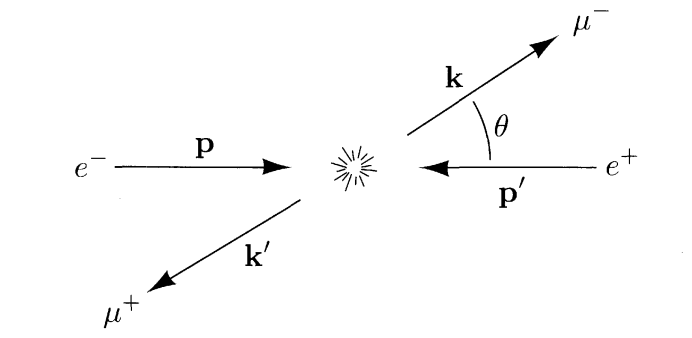
\includegraphics[width=0.6\textwidth]{trailer.png}
\caption{\label{trailer}\emph{electron positron annihilation}}
\end{figure}


\item The calculation we would like to perform is the differential cross section, that is the derivative of the cross section $\sigma$ with respect to the solid angle $\Omega$, $\frac{d \sigma}{d \Omega}$. This is a useful quantity as it is easily experimentally observed. In a particle collider, electrons and positrons are prepared in batches of length $l_A$ and $l_B$ and densities $\rho_A$ and $\rho_B$ respectively. When the two batches collide if the over lapping area of the head on collision is A, then the cross section is given by:
\end{itemize}

\begin{equation*}
  \sigma = \frac{\text{Number of events}}{\rho_A\rho_B l_A l_B A}
\end{equation*}

\begin{itemize}
  \item We now look at the dimensions of our quantities. Conveniently from our use of God given units, i.e. $\hbar =c =1$ we have that momentum, mass and energy have the same units as the energy mass equivalence becomes $E^2 = p^2 + m^2$. We also have from the Heisenberg's uncertainty principle that $\Delta p \Delta x \sim 1$. Thus the dimensions of mass and length are inversely related. 

  We can from this easily see that the dimensions of the quantity $[\rho_A\rho_B l_A l_B A]$ is $[m^2]$, which makes the dimensions of $\left[\frac{d\sigma}{d \Omega}\right] = \left[\frac{1}{m^2}\right]$ as angles are unitless. With this we can say that this quantity is also inversely proportional to the energy squared times some positive quantity that depends on the angle:


\begin{flalign}
\label{diff_cross}
  \frac{d\sigma}{d \Omega} \propto \frac{1}{E^2}|\mathcal{M}(\theta)|^2 
\end{flalign}
Here $\mathcal{M}$ is a dimensionless quantity, that is essentially the quantum mechanical amplitude for the process to occur. It does not depend on the energy $E$, as we are considering the limit where $E >> m_e,m_{\mu}$. This means we are unable to construct any dimensionless quantity like $E/m_e$ or $E/m_{\mu}$ as we have set $m_e/E = 0 = m_{\mu}/e$. Note that we could not take this limit and them $\mathcal{M}$ would depend on $E$, but it is simpler to consider the high energy limit. We will later calculate what the constant of proportionality in this equation is, and it turn out to be $1/64\pi^2$.
\end{itemize}
\begin{itemize}
  \item If we recall from Quantum mechanics, in perturbation theory we had that at first order the transition amplitude is related to the initial and final states along with the interaction Hamiltonian $H_i$, so:

\begin{equation*}
  \mathcal{M} \sim \bra{\text{final state}} H_I \ket{\text{initial state}}
\end{equation*}
But we know physically that the electrons do not interact with the muons, Instead what we know happens is that the electrons annihilate to form photons which in turn form the muons. This then means that $\bra{\mu^+ \mu^-} H_I \ket{e^+e^-} = 0 $ and instead we have that:

\begin{flalign}
\label{second order M}
  \mathcal{M} \sim \bra{\mu^+ \mu^-} H_I \ket{\gamma}^{\alpha}\bra{\gamma}H_I\ket{e^+e^-}_{\alpha}
\end{flalign}

This is a heuristic way of writing this second order contribution, but it makes sense physically as we have the electron positron pair interacting to become a photon ($\ket{\gamma}\bra{\gamma}$) and then the photon in turn becoming muons. Note the addition of vector indices ($\alpha$) as the photon is a vector particle (non-zero spin), so the photon created has 4 intermediate states, 3 for spin as it has spin-1 and one extra that comes from the fact that we are adding angular momenta in the four dimensional Lorentz group and must consider boosts also. (Remember the three spin components are generated by the three angular momentum operators and there is a corresponding generator for boosts). 
\end{itemize}

\begin{itemize}

  \item Since the photon must conserve angular momentum going to or from either of the two particles, the photon vector must be in the same direction as the axes of the particle pairs. We also know that the strength of the coupling between electrons (or muons) and photons is given by the electric charge $e$. This means for the case where electron has spin up along x axis, the positron has spin down:
\begin{equation*}
  \bra{\gamma} H_I \ket{e^+ e^-}^{\alpha} \propto e(0,1,i,0)
\end{equation*}
And if we have the same for muon and anti-muon:
\begin{equation*}
  \bra{\gamma} H_I \ket{\mu^+ \mu^-}^{\alpha} \propto e(0,\cos{\theta},i,-\sin(\theta))
\end{equation*}

The vectors here have the first component as the time component and the last three are part of the the polarization vector of the photon. See Jackson third edition page 299 for these vectors. 


\item When considering the experimental calculation of $\frac{d\sigma}{d \Omega}$ it also easier to account for all possible initial and final spin states, for which we need to take in to account conservation of angular momentum. This means we cant have two right polarized electron and positrons going to a left and right polarized muon and anti-muon. This condition then leaves 4 possible transitions which we can calculate the contributions. These calculations are done by dotting the two vectors we have above as in \ref{second order M}, making sure to take the complex conjugate of the first 4 vector and also remember to properly contract with the $(+---)$ metric. This results in:

\begin{flalign*}
& M(RL \rightarrow RL) \sim -e^2(1+\cos{\theta}) \\
& M(RL \rightarrow LR) \sim -e^2(1-\cos{\theta}) \\
& M(LR \rightarrow RL) \sim -e^2(1-\cos{\theta}) \\
& M(LR \rightarrow LR) \sim -e^2(1+\cos{\theta})
\end{flalign*}


There are no states that have 0 total angular momentum before and after as it turn out the intermediate photon (despite being a spin-1 boson) cant have spin 0 along an axis. Though in this case we would be requiring that the photon would have 0 total spin which is also not possible. 


\item We can finally take these 4 probabilities and square and sum them to get $|\mathcal{M}|^2$. Resulting in:

\begin{equation*}
  |\mathcal{M}|^2 \sim 4e^2(1+\cos^2{\theta})
\end{equation*}
So using \ref{diff_cross} and its proportionality constant $1/64\pi^2$ we can write:

\begin{equation*}
  \frac{d \sigma}{d \Omega} = \frac{e^2}{32E^2}(1+\cos^2{\theta})
\end{equation*}
Defining the constant $\alpha = e^2/4\pi \sim 137^{-1}$, we can then integrate this to get a expression for the total cross section as:

\begin{flalign*}
  \sigma = \frac{4\alpha^2\pi}{3E^2}
\end{flalign*}
This is the correct first order approximation!
\end{itemize}


\newpage  

\section{The need for Fields}
In this section we will see where regular quantum mechanics fails and what we need to do to fix it. 

\subsection{Non-relativistic free particle}

\begin{itemize}
  \item We can recall from QM that the probability of a particle at point $x$ at time $t$ propagating to $x'$ at time $t'$ is given by:
  \begin{equation}
  \label{propagator}
    \bra{x} e^{-iH(t-t')} \ket{x'}
  \end{equation}
  Here $H$ is the Hamiltonian. For a Non-relativistic free particle we have that $H = \hat{\textbf{P}}^2/2m$. We can then go about solving dor this propagator with this Hamiltonian in the usual way. This involves inserting the identity $\int \frac{d^3p}{(2\pi)^3}\ket{p}\bra{p} = \mathbb{I}$ into the above propagator \ref{propagator}before the $\ket{x'}$

  \begin{equation*}
      \bra{x} e^{-iH(t-t')} \ket{x'}  = \int \frac{d^3p}{(2\pi)^3}\bra{x}e^{-i\frac{\hat{\textbf{P}}^2}{2m}(t-t')}\ket{p}\braket{p|x'}
  \end{equation*}
  Then if we recall that $\braket{p|x'} = e^{-i\textbf{p}\cdot\textbf{x}'}$, $\braket{x|p} = e^{i\textbf{p}\cdot\textbf{x}}$ and $e^{-i\frac{\hat{\textbf{P}}^2}{2m}(t-t')}\ket{p} = e^{-i\frac{p^2}{2m}(t-t')}\ket{p}$. We get:

  \begin{flalign*}
    \bra{x} e^{-iH(t-t')} \ket{x'} & = \int \frac{d^3p}{(2\pi)^3}e^{-i\frac{p^2}{2m}(t-t')}e^{i\textbf{p}\cdot(\textbf{x}-\textbf{x}')} \\
    & = \left(\frac{m}{2\pi i(t-t')}\right)^{3/2}e^{im\frac{(\textbf{x}-\textbf{x}')^2}{2(t-t')}}
  \end{flalign*}
  \item What this is saying, is that for any two points $x$ and $x'$, no matter how far they are separated, have a non-zero probability of propagation from one to another. But this is direct contrast with what we know from special relativity! Two points separated by enough distance so that there space time interval, $\Delta s^2 = (t-t')^2 -|\textbf{x}-\textbf{x}'|^2$ is negative, i.e. space like. Which would require a propagation speed faster then light. 
\end{itemize}

\subsection*{Relativistic free particle}
\begin{itemize}
  \item But we can chalk this up to a mistake. We were not considering the Hamiltonian of a \textbf{relativistic} free particle. That is, with the Hamiltonian $H  = \sqrt{\textbf{P}^2 + m^2}$. The propagator in a similar manner to before then becomes: 
  \begin{equation*}
  \begin{split}
     \bra{x} e^{-i\sqrt{\textbf{P}^2 + m^2}(t-t')} \ket{x'} & = \int \braket{x|p}  e^{-i\sqrt{\textbf{P}^2 + m^2}(t-t')}  \braket{p|x'}\frac{d^3p}{(2\pi)^3} \\
     & = \int \frac{d^3p}{(2\pi)^3}  e^{-i\sqrt{p^2 + m^2}(t-t')+ i\textbf{p}\cdot(\textbf{x}-\textbf{x}')} 
  \end{split}
  \end{equation*}
  We can then parametrize the angle part of this integral by letting $\theta$ be the angle between $\textbf{p}$ and $(\textbf{x}-\textbf{x}')$, we can also further parametrize this with $\eta = \cos{\theta}$:
  \begin{equation*}
  \begin{split}
  \bra{x} e^{-i\sqrt{\hat{\textbf{P}}^2 + m^2}(t-t')} &\ket{x'}  = \int_{0}^{\infty} \frac{p^2dp}{(2\pi)^2}  \int_{-1}^{1} d \eta e^{-i\sqrt{p^2 + m^2}(t-t')+ ip|\textbf{x}-\textbf{x}'|\eta} \\
   = \int_{0}^{\infty} \frac{p^2dp}{(2\pi)^2}& e^{-i\sqrt{p^2 + m^2}(t-t')} \frac{1}{ip|\textbf{x}- \textbf{x}'|}\left(e^{ ip|\textbf{x}-\textbf{x}'|}-e^{- ip|\textbf{x}-\textbf{x}'|} \right)
  \end{split}
  \end{equation*}
  We can then turn this into an integral from $-\infty$ to $\infty$ with a factor of 2:
  \begin{equation}
  \label{Rel_propagator}
  \begin{split}
 = \frac{-i}{2\pi^2|\textbf{x}- \textbf{x}'|}\int_{0}^{\infty}pdp~e^{-i\sqrt{p^2 + m^2}(t-t')+ip|\textbf{x}-\textbf{x}'|}
  \end{split}
  \end{equation}
\end{itemize}
\subsubsection{Laplace steepest decent}
\begin{itemize}
  \item We can then use a useful approximation of integrals of this form by expanding around critical points. That is points $x_0$ where $f'(x_0)= 0$. The approximation is as follows, for a critical point $x_0$ of $f(x)$:
  \begin{flalign*}
\int_{-\infty}^{\infty}&h(x)e^{Af(x)}dx =  \int_{-\infty}^{\infty}h(x)e^{A\left[f(x_0) + \frac{1}{2}f''(x_0)(x-x_0)^2+\mathcal{O}((x-x_0)^3)\right]}dx \\ 
 \approx   h(x_0)e^{Af(x_0)}&\int_{-\infty}^{\infty}e^{-A\frac{1}{2}|f''(x_0)|(x-x_0)^2}dx = \sqrt{\frac{2\pi}{A|f''(x_0)|}}h(x_0)e^{Af(x_0)} 
  \end{flalign*}
  \item Where we have assumed $x_0$ is a global maxima so that $f''(x_0) \leq 0$. This approximation works well as the exponential ensures that any small deviation from $x_0$ contributes very little to the integral. It of course depends also on $h(x)$ being "well behaved".


  \item Back to the relevant integral \ref{Rel_propagator}, we can see that for us $f(p) = -i\sqrt{p^2 + m^2}(t-t')+ip|\textbf{x}-\textbf{x}'|$ and $h(p) = p$. So we find the stationary point of $f(p)$ via $f'(p_0)=0$: 
  \begin{equation*}
  \begin{split}
      f'(p_0) = \frac{-p_0(t-t')}{\sqrt{p_0^2+m^2}}+|\textbf{x}-\textbf{x}'| =0 \implies p_0^2 = \frac{m^2|\textbf{x}-\textbf{x}'|^2}{(t-t')^2-|\textbf{x}-\textbf{x}'|^2}
      \end{split}
    \end{equation*}  
    Then we can evaluate $f(p_0)$:
    \begin{equation*}
    \begin{split}
      f(p_0) & = -i\sqrt{\frac{m^2|\textbf{x}-\textbf{x}'|^2}{(t-t')^2-|\textbf{x}-\textbf{x}'|^2}+m^2}(t-t')+i\sqrt{\frac{m^2|\textbf{x}-\textbf{x}'|^2}{(t-t')^2-|\textbf{x}-\textbf{x}'|^2}} \\
      & = -\frac{m(|\textbf{x}-\textbf{x}'|^2-(t-t')^2)}{\sqrt{|\textbf{x}-\textbf{x}'|^2-(t-t')^2}} = -m\sqrt{|\textbf{x}-\textbf{x}'|^2-(t-t')^2}
    \end{split}
    \end{equation*}
    Where we have used the fact that we are considering probabilities outside the light-cone, i.e. where $|\textbf{x}-\textbf{x}'| > (t-t')$, so that the square root $ \sqrt{(t-t')^2-|\textbf{x}-\textbf{x}'|^2}=i\sqrt{|\textbf{x}-\textbf{x}'|^2-(t-t')^2}$ . 

    \item With this we can now use Laplace's steepest decent integral approximation to write:
    \begin{flalign*}
    \bra{x} e^{-i\sqrt{\hat{\textbf{P}}^2 + m^2}(t-t')} \ket{x'} \propto h(p_0)e^{f(p_0)} \propto e^{-\sqrt{|\textbf{x}-\textbf{x}'|^2-(t-t')^2}}
    \end{flalign*}
    This again does not solve our problem, we have that there is a non-zero probability of propagating to outside the light-cone. Some more radical approach is needed to solve this problem. 
\end{itemize}

\subsection{Field theory}
\begin{itemize}
  \item The  Idea will be to go from dealing with particle, to waves. For this we need to generalize our idea of action being the integral of a Lagrangian over time to being the integral of a Lagrange density over time and space as a field is spread out, not localized. This means:
  \begin{equation*}
    S = \int L(q_i,\dot{q}_i,t)dt \rightarrow \int d^4x\mathcal{L}(\varphi(\textbf{x},t),\partial_{\mu} \varphi(\textbf{x},t))
  \end{equation*}
  We then have to vary this action to set $\delta S = 0$:
  \begin{equation*}
    \delta S = \int d^4x \left(\frac{\delta \mathcal{L}}{\delta \varphi}\delta \varphi  - \frac{\delta \mathcal{L}}{\delta \partial_{\mu} \varphi}\delta\partial_{\mu}\varphi\right) = \int d^4x \left(\frac{\delta \mathcal{L}}{\delta \varphi}  - \partial_{\mu}\left(\frac{\delta \mathcal{L}}{\delta \partial_{\mu} \varphi}\right)\right)\delta \varphi 
  \end{equation*}
  \begin{flalign*}
    \implies \frac{\delta \mathcal{L}}{\delta \varphi}  - \partial_{\mu}\frac{\delta \mathcal{L}}{\delta \partial_{\mu} \varphi} = 0 
  \end{flalign*}
\end{itemize}



\end{document}
